% start: template for headers and footer info that need to be adde in each pade that includes a section
\chead{\textit{IT-University of Copenhagen} \rangle  SSEQ-E2013  \rangle \textbf{Group:} 10 Danish Travel card  \rangle \textbf{ID:} 46 \rangle Responsible: All}
\cfoot{\textbf{Hand-in date:} \today \rangle \textbf{Supervisor:} Marco Nardello \rangle \textbf{Version:} 1 \rangle \textbf{Status: } Done \thepage}
\renewcommand{\headrulewidth}{0.1pt}
\renewcommand{\footrulewidth}{0.1pt}
% ends: headers/footers template

\section*{Roles and Responsibilities}


\begin{figure}[ht!]
\centering
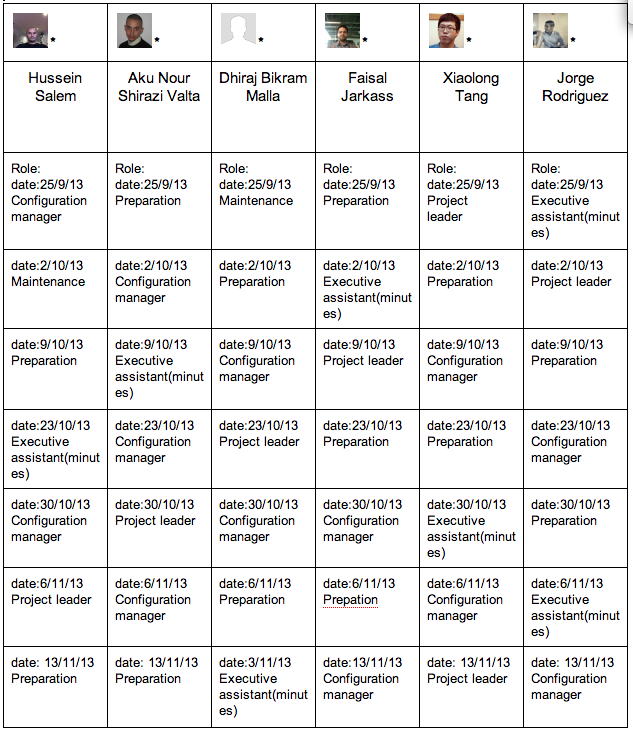
\includegraphics[width=100mm]{graphics/roles.png}
%\caption{Chapter 24 page 653}
\label{roles}
\end{figure}



\subsection*{Project Leader}
Leads the project for the particular week, which means that we chose a project leader each wednesday. And for that particular week, he is in charge of the work flow, and distributes the rest of the responsibilities to the rest of the team members. In addition he is the one controlling the group discussions. The project leader cannot overrule an earlier decision except if the majority of the group wishes to.


\subsection*{Preparation}
Preparation of supervisor meeting. Which mean that he is the one responsible for the meetings success. In order to get a productive meeting, the one in charge of this role has to prepare some questions for the TA. That means that he has to interact with all group members in order to collect all the doubts. This will lead to the agenda of the meeting.


\subsection*{Maintenance}
The maintenance responsible has to maintain the google drive, which means that he knows where the documents are placed and that they are placed in the correct directory.


\subsection*{Executive assistant}
The executive assistant takes minutes of the supervisor meeting and minutes of the group meetings, in order to collect all the information being discussed.
Prepare research documents for the particular week.


\subsection*{Configuration manager}
The configuration manager is responsible of the consistency of the developed documents. So that the changes are handled systematically. And keep track of the changes that are being made in the project.